\section{Encrypting content}

\section{Keys generation}
\subsection{Randomly derived}
  manual backup of the keys
\subsection{Keys derived from a password}

\section{Resilience against malicious nodes}

 \subsection{Reputation systems}
Reputation systems mitigate the problem of malicious nodes in
P2P networks, trying to build trust among the nodes. The key
idea of a reputation system is to predict the future behaviour
of nodes based on feedback about their past transactions [1]. A
transaction is application dependent, for example forwarding a
message in the network, buying an item in e-commerce services,
share or store files, etc. After a transaction, the client node emits
a recommendation that evaluates the behaviour of the other peer.
The aggregation of these recommendations leads to a reputation
value.
A reputation system built on top of a DHT has the ability
to compute a global reputation value for every node. Indeed
all the recommendations about a single node can be handled
consistently at a common location: either by a specific node
or by a set of nodes. Among existing reputation systems for
DHTs, we can cite: PeerTrust~\cite{peertrust}, WTR~\cite{wtr},
Eigentrust~\cite{eigentrust},
PowerTrust~\cite{powertrust} and CORPS~\cite{corps}

Reputation systems have to deal with malicious nodes that:
do not participate, collude with other malicious nodes and
emit false recommendations. There are techniques to mitigate
the impact of these attacks, such as the ones presented in
TrustGuard~\cite{trustguard} and WTR~\cite{wtr}. Nevertheless, to our knowledge,
none of the existing solutions to promote trust in P2P can be
$100\%$ effective in detecting and blocking these attacks.

It's assumed an $5\%$ error in the clasification of trusted nodes.


\paragraph{CORPS trust model}
They consider a probabilistic model of trust based on reputation.
The reputation value $R(X)$ is the probability that node $X$ will
be honest in the future. This reputation value is computed
according to a list of recommendations emitted by nodes that
have already carried out transactions with $X$.
After each transaction, a node emits a recommendation
about its peer. A node may lie: it may emit negative
recommendations about a peer that behaves correctly, or
positive recommendations about a malicious peer. Several nodes
may collude to increase or decrease the reputation value of
another node. These problems generate a deviation between
the computed reputation of the node and its real behaviour. It is
considered that this deviation depends on the function used to
compute the reputation value and on the percentage of malicious
nodes within the system.

It assumes a reputation system in the overlay structure with the following properties:
\begin{enumerate}
  \item Every node $X$ has an associated reputation value $R(X)$
  which represents the probability that $X$ is an honest node.
  \item $R(X)$ is computed using the recommendations emitted
  by nodes that have completed a transaction with $X$. Bad
  recommendations have a stronger effect on $R(X)$ than
  good ones. It should be more difficult for node to
  increase its reputation value than to decrease it.
  \item For every node $X$, $R(X)$ is highly available in the DHT.
\end{enumerate}

To avoid nodes that lie about a reputation value, it considers a reputation
system that computes the reputation of nodes concurrently on different nodes.
They decide individually if that node is reputable or not, using a voting
scheme in case of disagreement. On the whole, assuming that there is a smaller
percentage of malicious nodes in the network, the result avoids
false statements about reputation.

To maintain the same nomenclature used in CORPS, in all the following sections,
we call a node $n_i \in TS$ a trusted node, even if there still remains a
probability that this node's actual reputation is smaller than the threshold
$\rho$.
 
 
3.3 Self-Certification
A trusted authority issues identity certificates in a
centralized system. P. Dewan proposed a self-certification
mechanism [12] that splits the trusted entity among the
peers and enables them to generate their own identities in a
decentralized reputation system. Certified Authority (CA)
is run by each peer so as to issue an identity certificate(s)
for itself. These self certified certificates are similar to
SDSI certificates [9]. Each peer has its own reputation and
the reputations of all peers collectively form the reputation
of a CA.
In Self-certification mechanism there is no need for
centralized trusted entity which issues identities in a
centralized system. There is no way to map the identity of
a peer in the system to its real-life identity when they use
self-certified identities. They remain pseudonymous in the
system. The idea of making peers anonymous or
pseudonymous is desirable in P2P networks, but it can also
backfire sometimes.
In Self-certification mechanism the anonymity of the peers
is preserved by grouping of peers. The combination of self
certification and anonymity limits the possibility of a Sybil
attack. In contrast to the traditional CA-based approach,
neither the group authority nor the transacting peers can
establish the identity of the peer. In addition, certificate
revocations are not needed in the group-based approach as
the group authority only vouches for the real-life existence
of the peer, unlike the traditional certificate-based
approaches where various certificate attributes are attested
by the authority and necessitate revocation if any of those
attributes mutate in time. If a highly reputed identity is
compromised, its misuse would be self-destructive as its
reputation will go down if misused.

\chapter{Design of a username-password based identification system in structured P2P networks}

Existing systems for the user identification in P2P networks only consider the
use of preshared keys to identificate the user in the network. While that can
be easily implemented, does not provide to the users the flexibility that a
username-password based identification provides when using different devices to
log in in the system. As the user needs to transfer manually his keys from one
device to another, there are many security issues when they are handled without
care or the devices (like a cellphone) are lost. 

The use of a username and a password means that the user keys needs to be secured inside the identification system.
To handle the user keys without compromising the users identity, aditional
security layers needs to be placed inside the P2P network.

To secure the stored keys, the proposed system uses encryption, indirection and
rings of trust inside the network. The system goal is to offer a secure mean to
identify an user using only his username/password knowledge taking in
consideration the precense of bizantine nodes.

In this chapter we will describe the different parts of the system and how the
identification algorithms will work.
%In this section we describe the user identification system. 
%This system provides a distributed and secure way to attain a user-password
%identification scheme like the ones commonly seen in centralized services.

%\section{Securing  P2P networks}
\section{Securing storage in P2P networks}
P2P networks like gnutella,

% normal p2p networks provide storage for the peers inside but does not ensure
% control of capabilities, deletion nor modification of the files.

\section{Architectural principles}
%The general view of the system consists in a multi-layered network based in trusted rings.
The general view of the system consists in a double-layered network; a Trusted
ring of nodes nested inside a normal DHT, with multiple routing policies
depending in the protocol of differents services. The user registration,
sign-in, logout and password change operations respectively allow a node to
register an user identity, to identify himself with an existing user identity,
to remove your user session and to change the password used to sign-in.

The system needs to have a \textit{trusted ring} maintained by periodical
checks of capacity of his members to remain in the trusted ring and a
reputation system to evaluate this. Also, similar to the
leafset concept in Pastry, each trusted node needs to maintain a
\textit{trustset}, wich basically consist in D numerically closest trusted
nodes with D/2 clockwise nodes, and D/2 counter-clockwise ones.

The system used to build the trusted node infraestructure in the P2P networks
needs to regularly asses the ability of the nodes to be part of the trusted
ring.

The figure shows a basic structure of the system. There are normal nodes and
trusted nodes. Every trusted nodes maintains a \textit{trustsets}.

A simple storage system is needed.
The \textit{trustsets} are in charge of the storage of the user keys that are
used to identify an user in the system. The system needs a PUT(key,
file) operation that stores the file in the closest trusted node based in the
routing algorithm and a GET(key) operation that retrieves the stored file.


We now describe our protocols based on the system model. 
%Figure 2 shows the information objects and
%their storage locations, with arrows for the abstract flow of the
%login procedure, Table I lists the terms used in the algorithms.
%A. Account Registration

\section{Account registration}
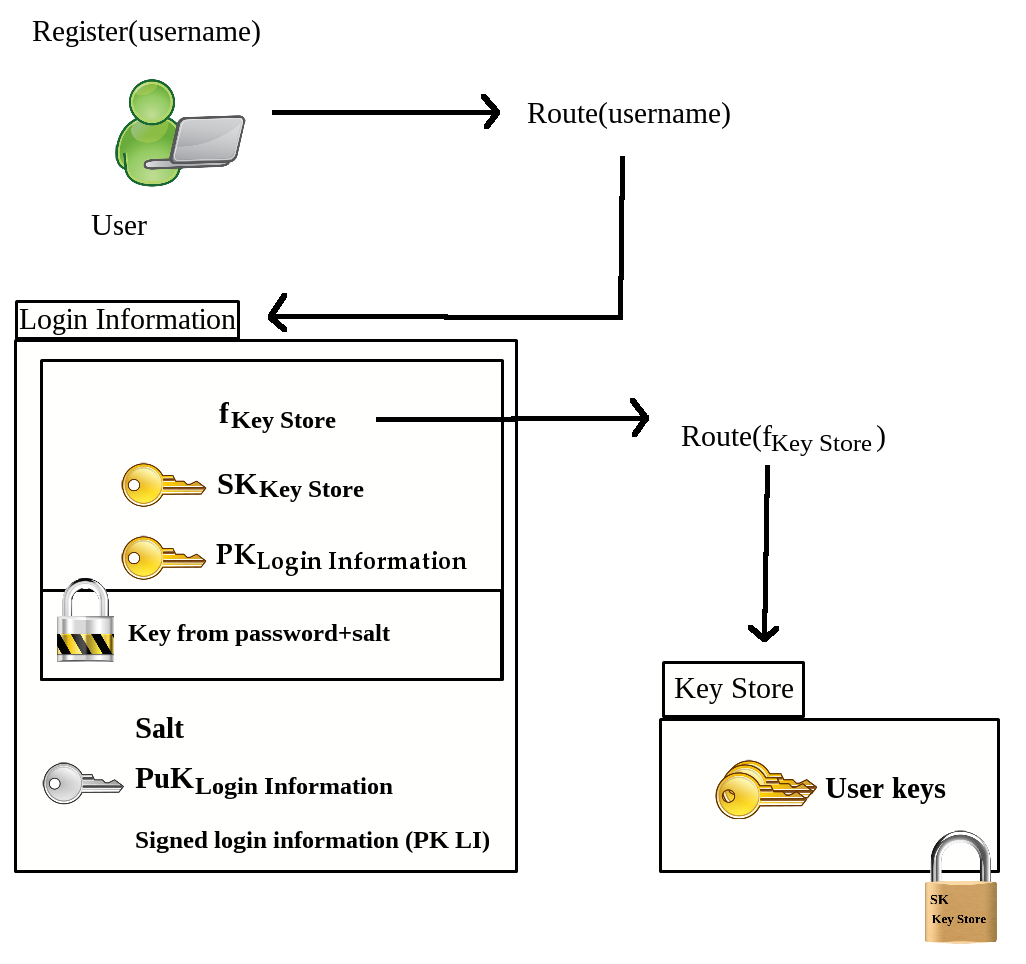
\includegraphics[width=14cm]{../img/user_registration}\\

To register a new user account, the user first
has to choose a \textit{username} and a \textit{password}.
%The \textit{username} should be unique in the network.
% The user checks if the username exists by sending a
% REGISTER(username, identity_file: [[c(user_keys_file), salt]).
% This operation use a accounted routing algorithm that uses only trusted
% nodes. When the register operation reaches the closest node to the username,
% it propagates a TRUSTSET_USERNAME_REGISTRATION operation. This operation sends a
% call to each node in the trustset of the node, wich then pass to do a council
% meeting. If the meeting results in favor, each of them sends a
% OK_USERNAME_REGISTRATION(user_identity_file_name) to node doing the REGISTER operation.
% 
% DETAILS OF THE REGISTER OPERATION
% DETAILS OF THE COUNCIL MEETING --> Explain before, in trusted node part 
% 

% key store file
Considering a key-based authentication, the user creates a \textit{key store file}, containing all the
keys used by the P2P application the user wants to log in to.
The user generates a cryptographic key to authenticate the write operations
that will be made in the file, and store this key along with the others in the
\textit{key store file}.


% encryption and store of the key store file
The user then creates a \textit{symmetric key KKS} ,
encrypts the file content with this key and puts the ciphertext
into the storage, obtaining a \textit{file name fKS} . Now, the user
creates a \textit{login information file} by creating a random
byte string \textit{salt}, deriving a \textit{symmetric key KLI} from the user
\textit{password} and the \textit{salt}.
Using the new \textit{ symmetric key KLI}, the user encrypts the \textit{file name fKS},
the \textit{symmetric key KKS} and the \textit{cryptographic key to
authenticate the write operations KW}.
 The salt and the three encrypted values are put
into the storage, obtaining a file name fLI . The salt is stored
in plaintext, so that the user later can derive the decryption
key KLI by only providing the password. Finally, the user
performs the write-once operation put on the DHT with
uname as key and fLI as value.

%unique username
If the username was taken,
the user is prompted for a new username.

%finish
Once all operations
have succeeded, the user is registered in the system.


\section{Sign-in}
The user uses his username to find and retrieve his \textit{login information
file}. Then, using his \textit{password} and the \textit{salt} included in the
\textit{login information file}, obtains the \textit{file name fKS} used to
route back to where the \textit{key store file} is stored.  Lastly, uses the
\textit{symmectric key KKS} to dencrypt the \textit{key store file} and recover
his user keys.

\section{Logout}
The system does not have something like a "session" to maintain; the only way
to identify an user is by his keys that are obtained by the identification
process.

%%%%%%%%%%%%%%% REWRITE THISSSSSSSSSSSSSSSSSSSSSSSSSSSSSSSS
 To log out from the system, the user does not have to interact
with the DHT or the storage system. Simply wiping her local
cache from application data and all key material restores the
pre-login state. If the user chose to remember the login on a
device, the corresponding device login information file FDL
can also be deleted from the storage.
 A problem related to logging out is revoking remembered
credentials on another device, e. g., a user’s stolen phone. To
accomplish this, we first run the password change operation,
which locks out all devices with remembered logins, because
he key store key KKS changed (as well as the filename fKS ).
Next, we use the device mapping devmap to inform all devices
about the new key (and filename), except the device that is to
be revoked. To inform a device about the change, we update
the corresponding values in the device’s login information file
 FDL which can be accessed from the device by using the
locally stored credentials.
 Algorithm 4 describes this necessary extension. After run- the password change
operation, all devices that not ning shouldbe revoked and that have remembered
logins (and therefore are devmap) referenced in the device mapping are
processed. The device login information filename fDL and its key KDL are read,
and the new key store key KKS new and filename fKS new are written to the
device login information file FDL, encrypted under the device key KDL.
Finally, the modified devmap is saved back to the login information file FLI.
%%%%%%%%%%%%%%% REWRITE THISSSSSSSSSSSSSSSSSSSSSSSSSSSSSSSS
 



\section{Password Change}
To change the password, the user has to rewrite his \textit{login information
file}.


%%%%%%%%%%%%%%% REWRITE THISSSSSSSSSSSSSSSSSSSSSSSSSSSSSSSS
Before the user can change the password, she must log in using her password to
obtain KLI . With this information, the password change can be accomplished
(see Algorithm 3): the user is asked for a new password and a new salt is
generated. The key-derivation function is used to generate a new key KLI new
for the login information file. Then, the content of the key-store file is
fetched and decrypted (with the old key). A new key KKS new is generated and
used for encrypting the key-store content again before it is saved to the
storage system, obtaining a new filename fKS new.
Finally, the login information file
is updated: fKS new, KKS new, the write credential KW as well as a new empty
device mapping devmapnew are encrypted with the new key KLI new.
  Together with the new salt, this ciphertext is written to the distributed
storage, using the reference fLI and the credential KW, to authenticate the
write operation. Lastly, the keys stored in the key store should be updated by
the application using our P2P protocol.  See Section VI-E for a discussion. At
this point, old device login information files can also be deleted from the
storage to reclaim space.
%%%%%%%%%%%%%%% REWRITE THISSSSSSSSSSSSSSSSSSSSSSSSSSSSSSSS


\chapter{Evaluation}

In this section we present a theoretical evaluation of
the authentication system.
%, as well as a set of simulations and performance
%results.

%%%Theoretical evaluation

We suppose in the following that the underlying
reputation system makes an error $\varepsilon$ when classifying a
node $X$ with a reputation $R(x) \geq \rho$, where $\rho \in [ 0 \cdots 1 ]$,
and $ \varepsilon = f ( \rho )$. In other words, classifying a node $X$ as
honest because its reputation is greater than $\rho$ has a
probability of error $\varepsilon$.
Let $n$ be the size of the Trusted Ring. The probability
to have $k$ misclassified nodes in the Trusted Ring, that
is $k$ malicious nodes is:

$$
P_{k_{malicious}} = \left(\!
                          \begin{array}{c}
                            n\\
                            k
                          \end{array}
                    \!\right)              
                    \varepsilon^{n-k} ( 1 - \varepsilon )^k
$$

Then, the probability to have at most $k$ malicious
nodes in a Trusted Ring of size $n$ is:

$$
P_{\leq k} = \sum^{k}_{i=1} \left(\!
                                \begin{array}{c}
                                    n\\
                                    k
                                  \end{array}
                            \!\right)              
                    \varepsilon^{n-i} ( 1 - \varepsilon )^i
$$

Therefore, the probability to have $k$ or more malicious
nodes in a Trusted Ring of size $n$ is:

$$
P_{\leq k} = \sum^{n}_{i=k} \left(\!
                                \begin{array}{c}
                                    n\\
                                    i
                                  \end{array}
                            \!\right)              
                    \varepsilon^{n-i} ( 1 - \varepsilon )^i
$$

The user identification fails when:
\begin{enumerate}
  \item The user cannot retrieve his own PKI from the \textit{trustset}.
  \item or when the public key of the user fails to be retrieved.
\end{enumerate}

These failures can happen when the \textit{trustsets} storing the PKI or the public
key have more malicious nodes than normal nodes.

The probability that a \textit{trustset} has half or more malicious nodes, assuming a maximum
classification error for the underlying reputation system
of $5\%$, is .% FILL HERE
%Hence the probability for having a fully erroneous trustset is theoretically possible, but
%practically infeasible.

Considering a maximum error rate of $5\%$ is a typical
value for a reputation system. In some cases it may be
over-estimated (for more details, please refer the results
obtained for the WTR reputation system\cite{wrt_reputation_system}). This
error hardly depends on the total number of malicious
nodes in the network, and decreases when the ratio
of malicious node decreases. The less malicious nodes
there are in the system, the easier it is to discriminate
against them.



\section{Forgotten passwords}

\section{Password-recovery mechanisms}
  - Security questions
  - threshold-based secret sharing with delegate selection and encrypting
  shares with passwords


%%%%%%%%%%%%%%% REWRITE THISSSSSSSSSSSSSSSSSSSSSSSSSSSSSSSS

An important part of password-based logins is the possi-
 bility for users to recover their accounts if they forget their
 passwords. We refer to this as a password recovery mechanism.
 The goal of a password recovery mechanism is to provide a
 secondary way of authenticating the user. There are a number
 of password recovery mechanisms used in practice. In our
 experience, three of the most common ones are password
 hints, security questions, and e-mail based recovery. Other

approaches (beyond the scope of this paper) include vouching
for identity by social contacts [21], or using trusted devices.
 Password hints means that the user may enter a hint at
the same time as she sets this password. The hint will be
displayed to her if she forgets her password, and should be
selected such that it helps her recall her password, but does
not make it significantly easier for someone else to guess it.
The hint is not truly a secondary authentication mechanism,
but rather a means to recovering the original password-based
authentication mechanism. A basic version of password hints
would be straightforward to implement in our system: the
hint can be stored in plaintext in the login information file.
Security questions and e-mail based password recovery are
more complex to adapt. We described their implementation in
detail after listing requirements.
 As in Section IV for the login procedure, we define a set of
functional requirements for password recovery, based on the
ISO 27002 standard [19] as follows. We also augment the list
with requirements of our own (preceded by a star).
establish methods to verify the identity of a user prior to
•allowing the user to choose a new password
communicate with those affected by or involved with
 - recovery security incidents
 - have procedures to allow recovery and restoration of
business operations and availability of information in a
 time-scaled manner
a legitimate user should be able to recover lost (forgotten)
 - or broken (device’s) keys
 - the recovery procedure should allow a user to set a new
 password, not reveal the old password
 - the process of recovery should be easy to use
 - sensitive information for recovery should be kept secret
Our protocols support these requirements. The sole exception
is that if a password is reset via security questions alone, the
system would not “communicate with those affected” (e.g.,
send an e-mail notification that the password had been reset,
as is common in centralized services). We remark that the
last item is a property many centralizedstronger than systems
provide. In our system, no one learns the answers to a user’s
security questions. We consider this to be important, since
many systems use similar security questions.
 The operations described in this section imply minor addi-
tions to the protocols of Section IV, i. e., invoking the update
procedures after each password change (to sustain transaction
safety, the updates have to be included in the final write
operation of the password change operation).
A. Security Questions
 Security questions is a password recovery technique that
relies on answers to questions the user is asked during regis-
tration. The answers should be such that they cannot be easily
guessed or researched by an attacker, but still stable over
time, memorable, and definite [22]. Rabkin [23] underlines
the importance to choose good questions especially in the era
of social networks. Frykholm and Juels [12] discuss a related
technique that is similar to our adaption of this scheme.

%%%%%%%%%%%%%%% REWRITE THISSSSSSSSSSSSSSSSSSSSSSSSSSSSSSSS

 

\section{Password Change}

